\section{Fases da missão de RVD/B}
\label{sec:fases_operacionais}

A sequência operacional foi dividida em fases, que se estendem desde a injeção orbital até o instante de captura.

\subsection{Injeção orbital inicial}

Após o lançamento, o veículo lançador insere o veículo visitante em uma órbita circular.
Nesse instante, o argumento de latitude do visitante do alvo são diferentes, por outro lado, os outros elementos orbitais de ambas as espaçonaves, como a excentricidade, inclinação, longitude do nodo ascendente e argumento do perigeu, são iguais.
Portanto, as diferenças iniciais entre o veículo visitante e o alvo se dão pelo argumento de latitude e por suas altitudes.

\begin{figure}[ht]
    \label{fig:injecao_orbita_inicial}
\centering
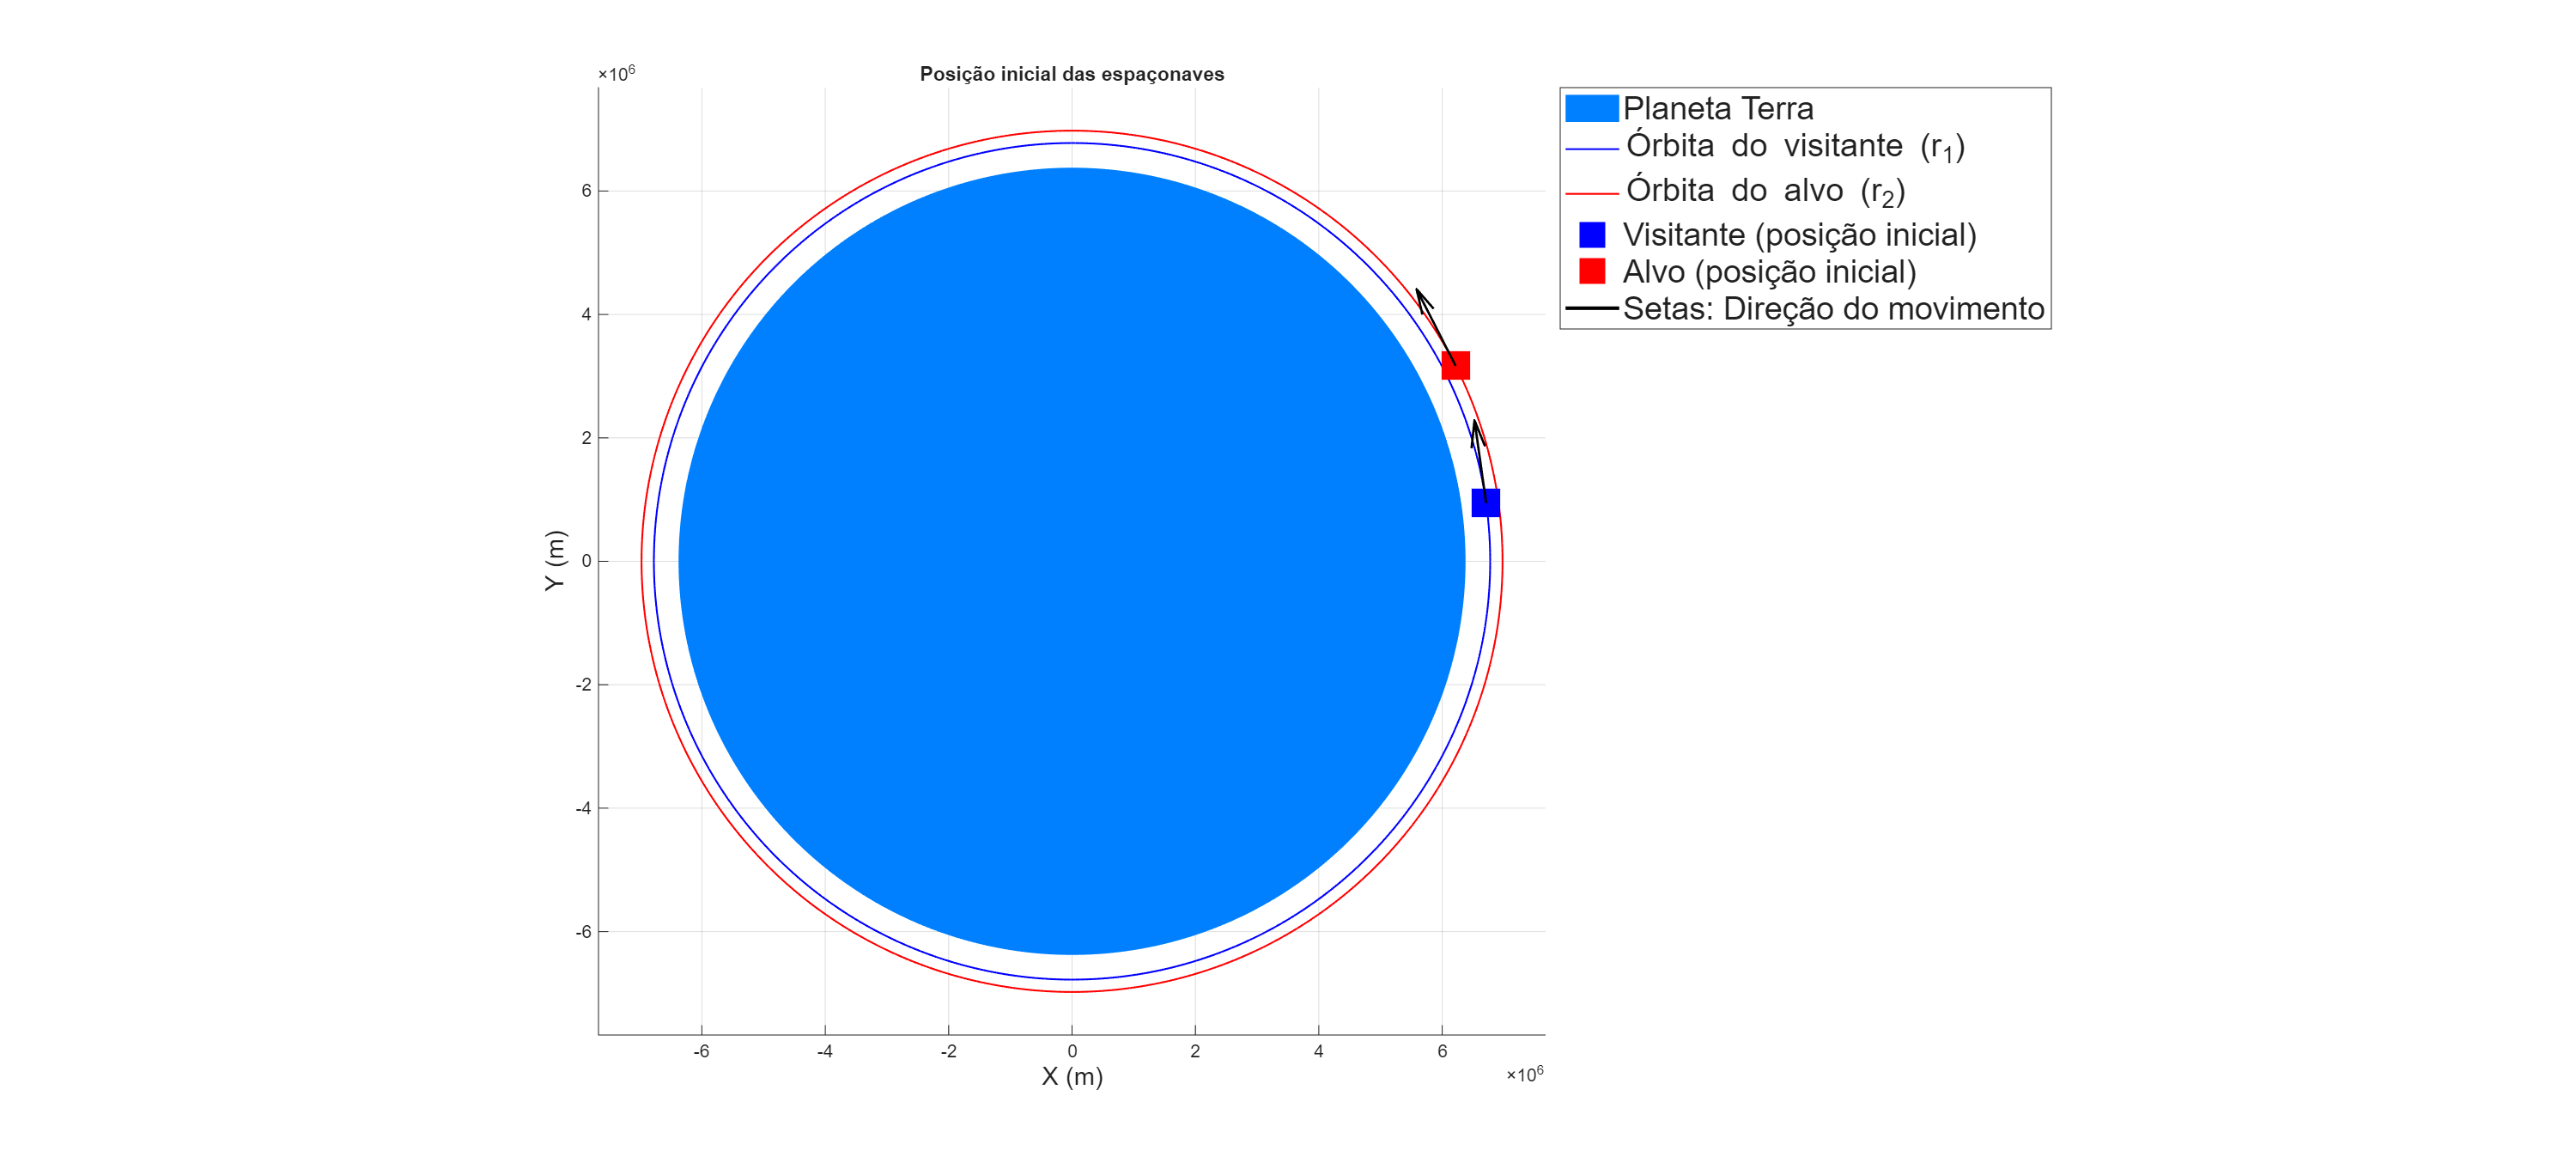
\includegraphics[width=1\linewidth]{3 Estrategia de RVDB/Imagens/1 Injecao orbita inicial.png}
\caption{Posição inicial das espaçonaves.}
\end{figure}

\subsection{Órbita de faseamento}  

Durante o faseamento orbital, o visitante ajusta sua posição ao longo de sua trajetória orbital para reduzir o ângulo de separação em relação ao alvo para executar a primeira manobra impulsiva da transferência de Hohmann.
Essa etapa é realizada de forma passiva, ou seja, não exige o consumo de propelente, exceto para manter a estabilidade orbital e a sincronização de atitude entre as espaçonaves.

\subsection{Transferência de Órbita}

São realizadas duas transferências de órbitas, a primeira para que o visitante saia de sua altitude inicial e estacione na órbita do alvo.
Neste momento os veículos possuem a mesma altitude.
A segunda transferência de órbita irá levar o visitante para uma altitude inferior à do alvo para iniciar a aproximação final.

\subsubsection{Primeira transferência de Hohmann}

A primeira transferência orbital é realizada por meio da transferência de Hohmann e resulta na elevação da altitude do visitante para a mesma altitude do alvo.
Após a execução dessa manobra, o visitante permanece no ponto de espera (\emph{hold point}) por cerca de duas horas.

\subsubsection{Ponto de espera}

O ponto de espera após a primeira transferência de Hohmann é utilizado para que a espaçonave visitante não ultrapasse ou fique atrasada em relação ao alvo; permite ainda que ele possa realizar checagens das velocidades absoluta e relativa, além das posições absoluta e relativa.
A altitude do ponto de espera é igual à altitude do alvo, no entanto, está localizado a uma distância entre 3000 e 4000 metros atrasado em relação à posição do alvo naquele instante.

\subsubsection{Segunda transferência de Hohmann}

Após concluir todas as verificações, o visitante realiza a segunda transferência de Hohmann, reduzindo sua altitude em relação à altitude do alvo.
Após se acomodar nesta posição orbital inicia-se a aproximação final, a qual predominam as manobras de controle fino.

\subsubsection{Aproximação final}
\label{sec:aproximacao_final}

Neste momento o veículo visitante se encontra nas proximidades da órbita do alvo, com velocidade relativa baixa e distância da ordem de dezenas de metros.
Ele permanece em \textit{modo de deriva} (\textit{drift}) até atingir o ponto apropriado, em relação ao alvo, para iniciar o deslocamento controlado ao longo do eixo radial do \textit{target}.

Durante essa movimentação, o controlador da espaçonave visitante executa pequenas correções de trajetória que resultam em um deslocamento em zigue-zague ao longo do eixo radial.
Esse padrão evita aproximações diretas e permite monitorar o alinhamento e a estabilidade relativa antes de entrar no corredor de aproximação final.

\subsubsection{Aproximação curta}
\label{sec:aproximacao_curta}

A aproximação curta ocorre nos últimos metros antes do acoplamento.
Nessa fase o visitante estende o manipulador robótico, abrindo as juntas revolutas e estende a junta prismática para acoplar a ferramenta à porta de docking do alvo.

\subsection{Pontos de referência}  

A cada fase da missão são definidos pontos de referência (\textit{waypoints}) que representam posições de verificação ou de troca de malha de controle.
A transição entre fases ocorre quando são satisfeitos os seguintes critérios:
  
\begin{enumerate}[label=(\roman*)]
\item distância relativa inferior a um limite pré-estabelecido para a etapa;
\item velocidade relativa inferior ao que foi definido para determinada etapa;
\item alinhamento angular relativo entre os eixos do referencial local de cada espaçonave estiverem dentro do limite estabelecido.
\end{enumerate}

\subsection{Sensores por fase}  
A Tabela~\ref{tab:sensores_fases} exibe os sensores empregados em cada etapa do processo de RVD/B.

\begin{table}[ht]
\centering
\caption{Sensores utilizados em cada fase da missão.}
\label{tab:sensores_fases}
\begin{tabular}{p{7cm} p{8cm}}
\toprule
\textbf{Fase} & \textbf{Sensor utilizado} \\
\midrule
Injeção orbital e faseamento& GPS e unidade inercial (IMU)\\
Transferências de Hohmann& GPS diferencial\\
Aproximação final e curta& LIDAR\\
Captura e acoplamento& LIDAR\\
\bottomrule
\end{tabular}
\end{table}

\subsection{Referencial}

Foi utilizado referenciais distintos pois cada fase da missão resolve um problema diferente.
Inicialmente, a dinâmica absoluta da órbita em torno da Terra e a dinâmica relativa entre visitante e alvo.
A escolha do referencial permite simplificar as equações, caso contrário exigira matrizes de transformação para cada etapa, o que ocasiona no incremento desnecessário de carga computacional; e tratando-se de espaçonaves, não costumam possuir poder computacional elevado.

\begin{table}[ht]
\centering
\caption{Referencial adotado em cada fase da missão.}
\label{tab:fases_tipo_ref}
\begin{tabular}{p{5cm} p{5cm} p{4cm}}
\toprule
\textbf{Fase da missão}& \textbf{Tipo} & \textbf{Referencial} \\
\midrule
Injeção orbital inicial& Movimento absoluto& ECI \\
Órbita de faseamento& Movimento absoluto& ECI \\
Transferência de órbita& Movimento absoluto& ECI \\
Aproximação final& Movimento relativo& LVLH \\
Aproximação curta& Movimento relativo& LVLH \\
\bottomrule
\end{tabular}
\end{table}
